% ETH Zurich  - 3D Photography 2015
% http://www.cvg.ethz.ch/teaching/3dphoto/
% Template for project proposals

\documentclass[11pt,a4paper,oneside,onecolumn]{IEEEtran}
\usepackage{graphicx}
% Enter the project title and your project supervisor here
\newcommand{\ProjectTitle}{3D Object Recognition with Deep Networks}
\newcommand{\ProjectSupervisor}{Martin Oswald, Pablo Speciale}
\newcommand{\DateOfReport}{March 7, 2015}

% Enter the team members' names and path to their photos. Comment / uncomment related definitions if the number of members are different than 2.
% Including photographs are optional. Photos are there to help us to evaluate your group more effectively. If you wish not to include your photos, please comment the following line.
\newcommand{\PutPhotos}{}
% Please include a clear photo of each member. (use pdf or png files for Latex to embed them in the document well)
\newcommand{\memberone}{Tobias Grundmann}
\newcommand{\memberonepicture}{pic1.png}
\newcommand{\membertwo}{Adrian Schneuwly}
\newcommand{\membertwopicture}{pic2.png}
\newcommand{\memberthree}{Johannes Oswald}
\newcommand{\memberthreepicture}{pic3.png}


%%%% DO NOT EDIT THE PART BELOW %%%%
\title{\ProjectTitle}
\author{3D Photography Project Proposal\\Supervised by: \ProjectSupervisor\\ \DateOfReport}
\begin{document}
\maketitle
\vspace{-1.5cm}\section*{Group Members}\vspace{0.3cm}
\begin{center}\begin{minipage}{\linewidth}\begin{center}
\begin{minipage}{3 cm}\begin{center}\memberone\ifdefined\PutPhotos\\\vspace{0.2cm}\includegraphics[height=3cm]{\memberonepicture}\fi\end{center}\end{minipage}
\ifdefined\membertwo\begin{minipage}{3 cm}\begin{center}\membertwo\ifdefined\PutPhotos\\\vspace{0.2cm}\includegraphics[height=3cm]{\membertwopicture}\fi\end{center}\end{minipage}\fi
\ifdefined\memberthree\begin{minipage}{3 cm}\begin{center}\memberthree\ifdefined\PutPhotos\\\vspace{0.2cm}\includegraphics[height=3cm]{\memberthreepicture}\fi\end{center}\end{minipage}\fi
\end{center}\end{minipage}\end{center}\vspace{0.3cm}
%%%% END OF PROTECTED LINES %%%%


%%%% BEGIN WRITING THE DOCUMENT HERE %%%%

\section{Description of the project}

The goal of this project is to successfully implement 3D object recognition using a Convolutional Neural Network (CNN) approach \cite{voxnet}. 
Such networks can be trained to recognize complex 3D shapes and determine the corresponding object class given a volumetric representation.
This project will mainly use the 3D CAD model data set called ModelNet \cite{wu}. Conceivably, volumetric data can also originate from 
inexpensive 2.5D depth sensors like Microsoft Kinect, Google Project Tango or Intel RealSense (Fig. \ref{fig:idea}).


% The main goal of our project is to enhance object recognition by making use of the recent availability of 2.5D  data through Microsoft Kinect, Google Project Tango, et al. 
%We will follow recent approaches \cite{wu}, \cite{voxnet} which use convolutional deep neural/belief networks to learn the distribution of complex 3D shapes across different object categories of CAD models. Given 2.5D data of a single view point, we will try to recognise the objects category after an intense training of our deep network on a large scale 3D CAD model dataset. Fig. \ref{fig:idea}

\begin{figure}
  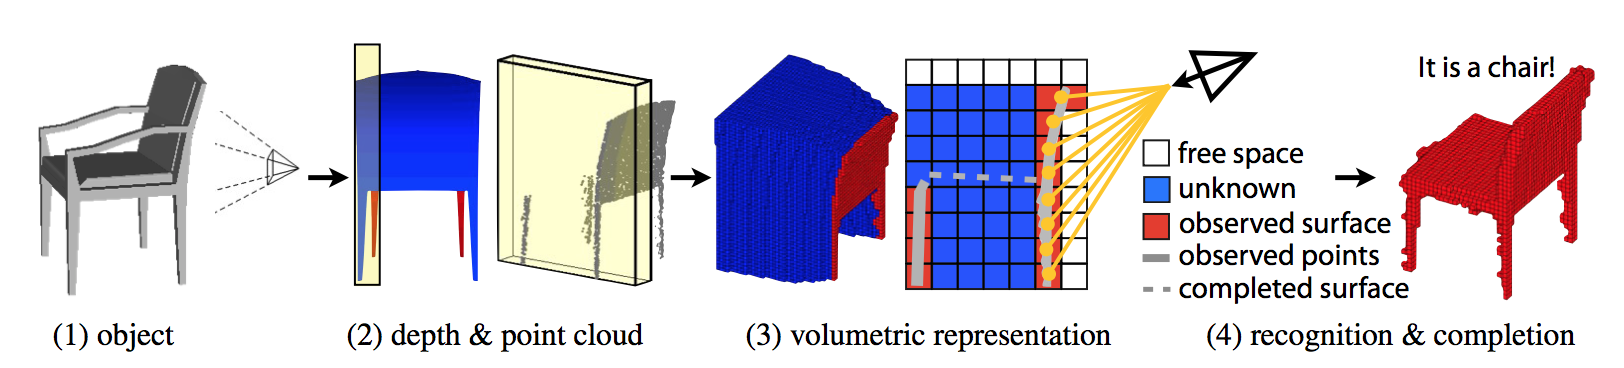
\includegraphics[width=\linewidth]{figure.jpg}
  \caption{2.5D object recognition}
  \label{fig:idea}
\end{figure}

\section{Work packages and timeline}

\subsection{Prerequisites in March}

The first goal of the team is to fully understand the approach described in \cite{voxnet}. Therefore everyone in the team works through the Udacity
deep learning course \cite{uda} individually in order to gain knowledge and hands-on experience with deep networks using 2D data.
Further, we get familiar with TensorFlow\footnote{open source library for machine intelligence} (in Python), which is used to implement the network architecture. 
As a first simple exercise to approach the problem we reproduce the character recognition example \cite{mnist} using the MNIST data set. 
In order to gain experience for the 3D case, we further extend that example and make it rotation invariant.
%In a next step, we will extend that example and make it rotation invariant to gain experience for the 3D case. \newline

The division of work among the 3 project members will happen after this initial project phase, because at this point in time it is hard to foresee how 
the work could be split meaningfully. 


\subsection{Modeling \& Data Preparation in April}

We begin implementing the VoxNet Convolutional Neural Network architecture \cite{voxnet} in Python while using the framework provided by the Udacity deep learning course \cite{uda}
as a base. Once the basic network is performing well, rotation invariance is added using the approach described in \cite{voxnet}.
The input to the network is a small voxel volume (30x30x30) and the output is an object class. 
Part of the ModelNet is already provided in volumetric representation. If necessary, additional CAD models can be converted to a voxel data structure 
using the Matlab script provided by \cite{wu}. 

% This for example enables the usage of real Google Tango data for object recognition testing.


% The available data is split into 3 part, namely a training, evaluation and testing set.


% 
% Good deep network performance heavily depends on extensive data sets. Therefore we are going to use the ModelNet dataset from \cite{wu}, a CAD dataset of 660 categories. 
% The datasets will 
% 
% First with ModelNet40, which is voxelized.
% 
% Unless we decide to use real tango data
% 
% transformed into 32x32x32 voxel data and split into a training, valuation and test set. If possible we will use data from the project tango tablet to cross test. 
% 
% We begin reimplementing the VoxNet Deep Convolutional Neural Network approaches in Python by starting with the deep learning udacity courses framework. \cite{uda} 
% Therefore we will remodel the given 2D object recognition network into a rotation-invariant 3D recognition network which makes heavily use of convolution and pooling. 
% The output of the deep network is the the class of object the network thinks it recognized from the input.


\subsection{Training \& Testing in June}
After the  successful implementation, we train the deep network with the ModelNet40 data set, which consists of 40 common categories with 
100 unique CAD models per category (voxel format). The data is split into two parts, namely a training and testing set. For the network training only
the training set is used. In this phase we fiddle around with network parameters while constantly evaluating the performance.
Due to the computationally expensive nature of the training, we expect this process to be time consuming. 



\section{Outcomes and Demonstration}

Goal of the project is to build up the VoxNet \cite{voxnet} architecture and train the network to recognize objects.
We hope to achieve similar positive recognition results as described in the paper \cite{voxnet}. 
In the live demo, we feed the network with data from the testing set (ModelNet40) or possibly real Google Tango data and 
then try to classify the objects.

% An advanced goal, is to possibly even use real Google Tango data try to classify objects (e.g chair).

% 
% 
% Goal of the project is to build up the VoxNet \cite{voxnet} architecture and train the network to recognize the objects
% rotation invariant. We hope to achieve similar positive object recognition results as described in the paper. 
% 
% re-implement the papers approach for 3D Object Recognition and achieve very similar positive object recognition results. 
% Rotational invariant
% 
% In the live demo, we will feed the algorithm randomly chosen CAD Models and try to classify the objects. 
% 
% % possibly use real tango data which requires an additional step of voxelization 


\vspace{1cm}

{%\singlespace
{\small
\bibliography{refs}
\bibliographystyle{plain}}}




\end{document}
